% !TeX root = main.tex
\section{Videos Submitted}

The videos can be found \href{https://iiitaphyd-my.sharepoint.com/:f:/g/personal/avneesh_mishra_research_iiit_ac_in/EogE243Ab4lDvm5VSueCLY8B7tLHOWnVw8i8PQnv5Bndfg?e=k8xJ1n}{here} (link: \url{https://iiitaphyd-my.sharepoint.com/:f:/g/personal/avneesh_mishra_research_iiit_ac_in/EogE243Ab4lDvm5VSueCLY8B7tLHOWnVw8i8PQnv5Bndfg?e=k8xJ1n}).

\subsection{Case 1}

File name is \texttt{out\_1.avi} (trajectories in figure \ref{fig:case-1-traj}). The case uses \texttt{single\_wpt\_path.py} and has the following configurations.

\begin{lstlisting}[language=Python, numbers=none]
    # ==== Begin: User configuration area ====
    # Points as [x, y]
    start_pt = [0, 0]
    end_pt = [40, 40]
    way_pt = [5, 30]
    # Time values
    to, tw, tf = [0, 20, 50]    # Start, waypoint, end
    # Other parameters
    ko, kw, kf = [0, np.tan(np.pi/5), 0]    # k = np.tan(theta)
    dko, dkw, dkf = [0, 0, 0]
    dxo, dxw, dxf = [0, 0, 0]
    # ==== End: User configuration area ====
\end{lstlisting}

\begin{figure}[ht]
    \centering
    \begin{subfigure}[b]{0.3\textwidth}
        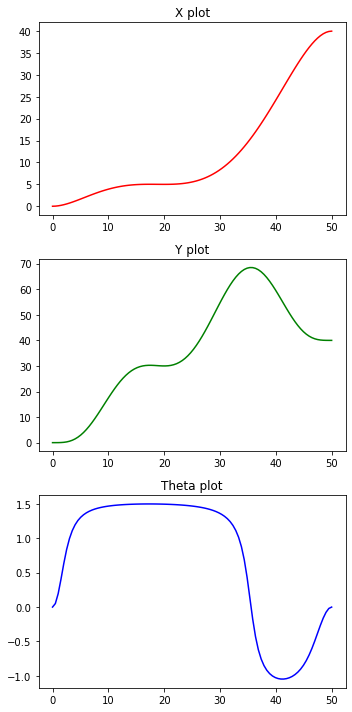
\includegraphics[width=\textwidth]{out-1.png}
        \caption{Plots for $x$, $y$, and $\theta$}
    \end{subfigure}
    \begin{subfigure}[b]{0.6\textwidth}
        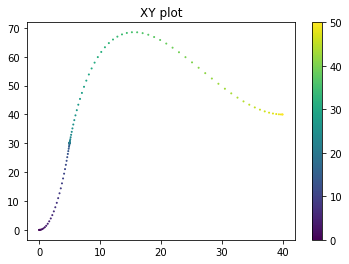
\includegraphics[width=\textwidth]{out-1-xy.png}
        \caption{Plot for $x, y$ path}
    \end{subfigure}
    \caption{Case 1 trajectories}
    \label{fig:case-1-traj}
\end{figure}

\paragraph*{Observations}
As it can be seen, the constraints for the `dx` at waypoint is being adhered (the vehicle comes to a stop there). It'll be more beneficial to not stop at waypoints.

\subsection{Case 2}

File name is \texttt{out\_2.avi} (trajectories in figure \ref{fig:case-2-traj}). The case uses \texttt{single\_wpt\_path.py} and has the following configurations.

\begin{lstlisting}[language=Python, numbers=none]
    # ==== Begin: User configuration area ====
    # Points as [x, y]
    start_pt = [0, 0]
    end_pt = [40, 40]
    way_pt = [10, 20]
    # Time values
    to, tw, tf = [0, 20, 50]    # Start, waypoint, end
    # Other parameters
    ko, kw, kf = [0, np.tan(np.pi/5), 0]    # k = np.tan(theta)
    dko, dkw, dkf = [0, 0, 0]
    dxo, dxw, dxf = [0, 1, 0]
    # ==== End: User configuration area ====
\end{lstlisting}

\begin{figure}[ht]
    \centering
    \begin{subfigure}[b]{0.3\textwidth}
        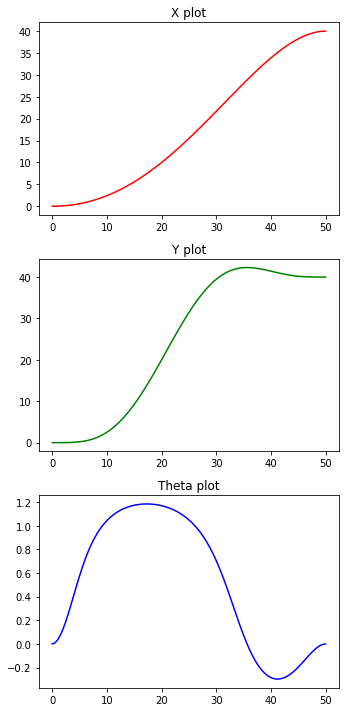
\includegraphics[width=\textwidth]{out-2.png}
        \caption{Plots for $x$, $y$, and $\theta$}
    \end{subfigure}
    \begin{subfigure}[b]{0.6\textwidth}
        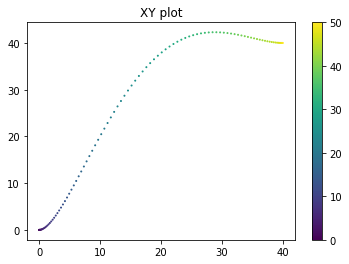
\includegraphics[width=\textwidth]{out-2-xy.png}
        \caption{Plot for $x, y$ path}
    \end{subfigure}
    \caption{Case 2 trajectories}
    \label{fig:case-2-traj}
\end{figure}

\paragraph*{Observations}
Here, the vehicle doesn't stop at the waypoints and this makes the overall curve much better. Let's see observations when the $\theta$ is not zero at starting and ending.

\subsection{Case 3}

File name is \texttt{out\_3.avi} (trajectories in figure \ref{fig:case-3-traj}). The case uses \texttt{single\_wpt\_path.py} and has the following configurations.

\begin{lstlisting}[language=Python, numbers=none]
    # ==== Begin: User configuration area ====
    # Points as [x, y]
    start_pt = [0, 0]
    end_pt = [50, 40]
    way_pt = [35, 10]
    # Time values
    to, tw, tf = [0, 30, 50]    # Start, waypoint, end
    # Other parameters
    ko, kw, kf = [np.tan(np.deg2rad(45)), 
        np.tan(np.pi/5), 
        np.tan(np.deg2rad(80))]    # k = np.tan(theta)
    dko, dkw, dkf = [0, 0, 0]
    dxo, dxw, dxf = [0, 1, 0]
    # ==== End: User configuration area ====
\end{lstlisting}

\begin{figure}[ht]
    \centering
    \begin{subfigure}[b]{0.3\textwidth}
        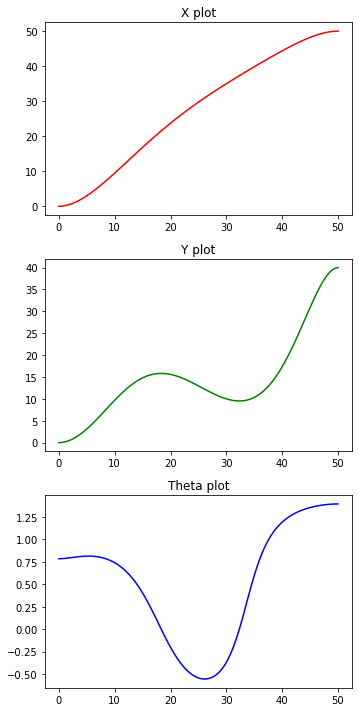
\includegraphics[width=\textwidth]{out-3.png}
        \caption{Plots for $x$, $y$, and $\theta$}
    \end{subfigure}
    \begin{subfigure}[b]{0.6\textwidth}
        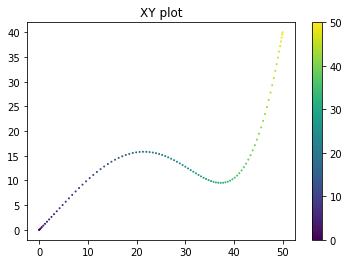
\includegraphics[width=\textwidth]{out-3-xy.png}
        \caption{Plot for $x, y$ path}
    \end{subfigure}
    \caption{Case 3 trajectories}
    \label{fig:case-3-traj}
\end{figure}

\paragraph*{Observations}
Here, the vehicle starts and ends with an angle other than zero. This makes tha curve better conditioned and there is very little overshoot. It also has a very nice curve to reach the waypoint and be back to the goal.
